In Fig.~\ref{fig:wg1_mjj-llLO}, we show the distributions in the invariant mass (top) and the rapidity difference of the two tagging jets (bottom) which are key observables for VBS measurements.
In both cases we show the absolute distributions in the upper plot, while the lower plot displays the ratio over {\sc VBFNLO} \MP{To be changed to Recola}.
For both observables we find a relatively good agreement among the various tools, which confirms the fact that contributions from $s$-channel diagrams as well as from non-resonant configurations are suppressed in the fiducial region.
In general, the agreement is at the level of $1\%$ or below for each bin.
We have checked that the same level of agreement holds for other standard differential distributions such as rapidity, invariant mass, or transverse momentum.
This means that at LO, in the fiducial volume and for energies relevant to the LHC, the VBS approximation is good to a per cent.
This is in agreement with the findings of section \ref{subsec:LOinclusive} as the present comparison completely excludes the region where tri-boson contributions could have a noticeable impact.

 \begin{figure*}[htb!]
   \centering
   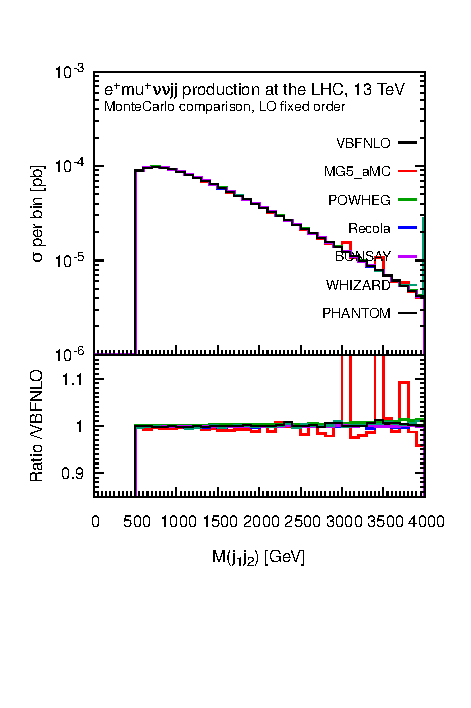
\includegraphics[width=0.4\textwidth,angle=0,clip=true,trim={0.4cm 2cm 0.cm 1.cm}]{figures/LO/mjj_LO.pdf}
   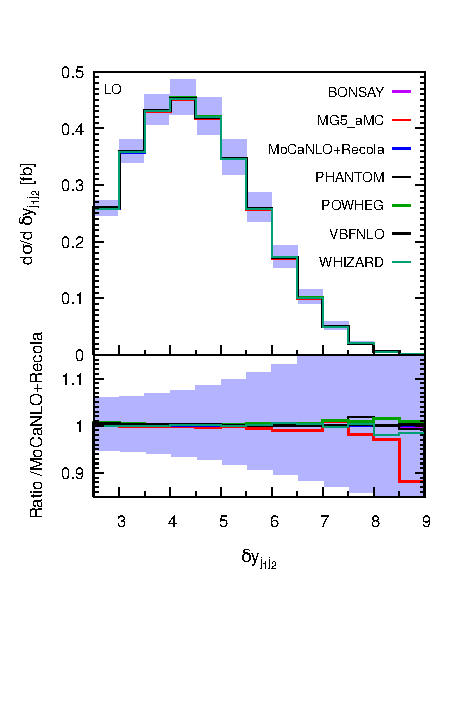
\includegraphics[width=0.4\textwidth,angle=0,clip=true,trim={0.4cm 2cm 0.cm 1.cm}]{figures/LO/dyj1j2_LO.pdf}
\caption{\label{fig:wg1_mjj-llLO} Differential distributions in the invariant mass (left) and rapidity difference of the two tagging jets (right).
The LHC process considered is ${\rm p}{\rm p}\to\mu^+\nu_\mu{\rm e}^+\nu_{\rm e}{\rm j}{\rm j}$ at LO accuracy and order $\mathcal{O}(\alpha^6)$.
The description of the different programs used can be found in Sec.~\ref{subsec:codedescr}.
The upper plots provides the absolute value for each prediction while the lower plots presents all predictions normalised to {\sc MoCaNLO}+{\sc Recola} which is one of the full predictions.
The predictions are obtained in the fiducial region described in Sec.~\ref{subsec:inputpar}.
\MP{MG statistics should be improved and the baseline changed to Recola.}
}
\end{figure*}
